\documentclass[12pt]{article}
\usepackage[verbose=true,letterpaper]{geometry}
\usepackage{amsmath}
\AtBeginDocument{
	\newgeometry{
		textheight=8.6in,
		textwidth=7.0in,
		top=1in,
		headheight=14pt,
		headsep=25pt,
		footskip=30pt
	}
}

\widowpenalty=10000
\clubpenalty=10000
\flushbottom
\sloppy

\usepackage{fancyhdr}
\fancyhf{}
\pagestyle{fancy}
\renewcommand{\headrulewidth}{0pt}
\fancyheadoffset{0pt}
%\fancyhead[LE,RO]{\thesection}
\fancyhead[RE,LO]{\leftmark\vspace{5pt}}
\cfoot{\vspace{5pt}\thepage}
\renewcommand{\headrulewidth}{1pt}
%\renewcommand{\footrulewidth}{1pt}


\usepackage[utf8]{inputenc} % allow utf-8 input
\usepackage[T1]{fontenc}    % use 8-bit T1 fonts
\usepackage{hyperref}       % hyperlinks
\usepackage{url}            % simple URL typesetting
\usepackage{booktabs}       % professional-quality tables
\usepackage{amsfonts}       % blackboard math symbols
\usepackage{nicefrac}       % compact symbols for 1/2, etc.
\usepackage{microtype}      % microtypography
\usepackage{lipsum}
\usepackage[utf8]{inputenc} % Required for inputting international characters
\usepackage[T1]{fontenc} % Output font encoding for international characters
\usepackage{graphicx}
\usepackage{mathpazo} % Palatino font
\hypersetup{%
	pdfborder = {0 0 0}
}

\graphicspath{ {./images/} }

\usepackage{enumitem}
\setlist{nosep}

\usepackage{setspace}
%\singlespacing
\onehalfspacing
%\doublespacing
%\setstretch{1.1}

\begin{document}


\begin{titlepage} % Suppresses displaying the page number on the title page and the subsequent page counts as page 1
	\newcommand{\HRule}{\rule{\linewidth}{0.5mm}} % Defines a new command for horizontal lines, change thickness here
	
	
	
	\center % Centre everything on the page
	
	%------------------------------------------------
	%	Headings
	%------------------------------------------------
	
	%\textsc{\LARGE Deutsche Bank}\\[0.5cm] % Main heading such as the name of your university/college
	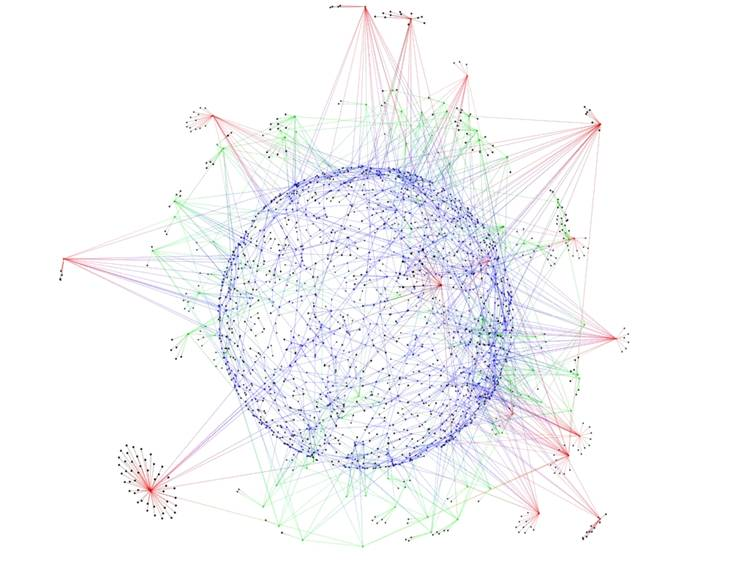
\includegraphics[scale=1]{PPI.jpg}\\[1cm]
	
	%\textsc{\huge Major Heading}\\[0.5cm] % Major heading such as course name
	
	%\textsc{\large Minor Heading}\\[0.5cm] % Minor heading such as course title
	
	%------------------------------------------------
	%	Title
	%------------------------------------------------
	
	\HRule\\[0.5cm]
	
	\huge \textsc{\textbf{Introduction to the Statistics of Financial Derivatives}}\\[0.01cm] % Title of your document
	
	\HRule\\[1.0cm]
	
	%------------------------------------------------
	%	Author(s)
	%------------------------------------------------
	
	\vfill\vfill\vfill
		\large
	\textsc{Author}\\
	\small {\textbf{Ali Al-Hayki}\\
		Valuations \& Risk Management\\
		Deutsche Bank\\
		\texttt{ali.hayki@gmail.com} \\
		\texttt{ali.al-hayki@db.com} \\}
	
	
	% If you don't want a supervisor, uncomment the two lines below and comment the code above
	%{\large\textit{Author}}\\
	%John \textsc{Smith} % Your name
	
	%------------------------------------------------
	%	Date
	%------------------------------------------------
	
	\vfill\vfill\vfill % Position the date 3/4 down the remaining page
	
	{\large\today} % Date, change the \today to a set date if you want to be precise
	
	%------------------------------------------------
	%	Logo
	%------------------------------------------------
	
	%\vfill\vfill
	%\includegraphics[width=0.2\textwidth]{placeholder.jpg}\\[1cm] % Include a department/university logo - this will require the graphicx package
	
	%----------------------------------------------------------------------------------------
	
	\vfill % Push the date up 1/4 of the remaining page
	
\end{titlepage}


\tableofcontents
\newpage
\listoffigures
\newpage
\listoftables
\newpage



\begin{abstract}
	\lipsum[1]
\end{abstract}

\setlength{\parindent}{0em}
\setlength{\parskip}{0.5em}
\renewcommand{\baselinestretch}{0.01}
\newcommand{\R}{\mathbb{R}}
\newcommand{\B}{\mathbb{B}}
\newcommand{\C}{\mathbb{C}}
\section{Set Theory}
\subsection{Sets and Members}
A set is a well-defined collection of objects. The objects of a set are called elements or members. The elements of a set can be anything: numbers, people, letters of the alphabet, other sets, and so on. The elements contained in a given set need not have anything in common (other than the obvious common attribute that they all belong to the given set). Equally, there is no restriction on the number of elements allowed in a set; there may be an infinite number, a finite number, or even no elements
at all. There is, however, one restriction we insist upon: given a set and an object, we should be able to decide (in principle at least — it may be difficult in practice) whether or not the object belongs to the set. This is what we meant above by a ‘well-defined’ collection: given an object a and a set A, it must be unambiguous whether or not a belongs to A.

Sets are conventionally denoted with capital letters, $A, B, C, etc$. Two sets A and B are said to be equal, written $A=B$, if they have the same members. A set can also have zero members. Such a set is called the \textbf{empty} set (or the \textbf{null} set) and is denoted by $\phi$.

If every member of the set A is also a member of the set B, then A is said to be a subset of B, written $A \subset B$, also pronounced A is contained in B.

\textbf{Set Notations and Operations:}

Let \textit{A, B} $A_n, n=1,2,...,$ denote subsets of the set $\Omega$

The symbol $\in$ denotes \textit{'belongs to'} or \textit{'is an element of'}. Thus

\begin{itemize}
	\item $x \in A \Longleftrightarrow$ the element \textit{a} belongs to (the set) \textit{A}
	
	\item $x \notin A \Longleftrightarrow$ means $\neg(x \in A)$ \textit{a} belongs to (the set) \textit{A}
\end{itemize}

\begin{itemize}
	\item 
\end{itemize}

\begin{itemize}
	\item \textit{Union: }Let A and B be any two sets. The set which consists of all the points which are in A or B or both is defined the Union and is written $A \cup B$.
	\item \textit{Intersection: }Let A and B be any two sets. The set that consists of all the points which are both in A and B is defined the intersection and is written $A \cap B$ or AB.
	\item \textit{Disjoint: }Let $A_1,A_2, \cdots A_n \subset$ U. It is said that a set is disjointed if $A_i \cap A_j=\phi$ for any $i,j.$
\end{itemize}
\subsection{Defining Sets}

Sets can be defined in various ways. The simplest is by listing the elements enclosed between curly brackets or ‘braces’ { }. Examples:

\begin{enumerate}
	\item $A=\{'Larissa', 'Bambulka', 'London',\}$ - This is the rather odd set containing three elements described above.
	\item $B=\{2,4,6,8,...\}$ - This is the infinite set described above. We clearly cannot list all the elements. Instead we list enough elements to establish a pattern and use '...' to indicate that the list continues indefinitely.
	\item $C=\{1,\{1,2\}\}$ - This set has 2 
	
	
	
\end{enumerate}

\subsection{Open Sets, Closed Sets  and Complements}
A set U is called \textbf{open} if, intuitively speaking, you can 'wiggle' or 'change' any point x in U by a small amount in any direction and still be in inside U. In other words, if x is surrounded only by elements of U; it can't be on the edge of U.

As a typical example, consider the open interval (0,1) consisting of all real numbers x with $0<x<1$. If you 'wiggle' such an x a little bit (but not too much), then the wiggled version will still be a number between 0 and 1. Therefore, the interval (0,1) is open.

However, the interval (0,1] consisting of all numbers x with $0<x\leq1$ is not open; if you take $x=1$ and wiggle a tiny bit in the positive direction, you will be outside of (0,1].

If A $\subset$ U then the complement of A in U, denoted by $A^c$, or $\bar{A}$ is:

\begin{equation}
A^c=U-A
\end{equation}
A \textbf{closed} set is a set whose complement is open. The real line $\mathcal{R}$, is both an open and a closed set.
\subsection{$\sigma$- algebra}

A $\sigma$- algebra (or $\sigma$- field) over a set X is a family of subsets of X that is closed under countable set operations 
\footnote{A set is closed under an operation if you can apply that operation to any combination of elements in the set and still have the resulting element in the set. For example A set is closed under (scalar) multiplication if you can multiply any two elements, and the result is still a number in the set. For instance, the set $\{1,-1\}$ is closed under multiplication but not addition. I generally see 'closed under some operation' as the elements of the set not being able to "escape" the set using that operation.} (union, intersection, complements); 
$\sigma$- algebra are mainly used in order to define measures on X. More formally, Consider the collection of set $\Omega$. Then, $\mathcal{B}$ is a $\sigma$-algebra if:

\begin{enumerate}
	\item $\Omega \in \mathcal{B}$
	\item $B \in \mathcal{B}$ implies $B^C \in \mathcal{B}$
	\item $B_{i}, i \geq 1$ implies $\bigcup^{\infty}_{i=1}$
\end{enumerate}

A very important $\sigma$- algebra is the Borel $\sigma$- algebra. Consider $\mathcal{R}$, the real line $\mathcal{C} =\{(a,b],-\infty\leq a \leq b \leq+\infty\}$, intervals that are open to the left and closed to the right.

\subsection{Function}
A function is a relation, such that each element f a set (the domain) is associated with a unique element of another (possibly the same) set (the codomain). We denote:

\begin{equation}
f:domain \longrightarrow codomain
\end{equation}

The most important functions for our purposes are the density and distribution functions, which we will introduce below.
\section{Probability Theory}

\subsection{Probability System}

We need to acquire an understanding of the different parts of a probability system and how they fit together. In order to make some sense of it all, we shall find it useful to think of a probability system as a physical experiment with a random outcome. To be more concrete, we shall use a special example to guide us through the various definitions and what they signify.

Suppose that we toss a coin three times and record the results in order. This is a very simple experiment, but note that we should not necessarily assume that the coin toss is fair, with an equally likely outcome for heads or tails. There can, in principle, be many different probabilities associated with the same 'physical experiment'. This will have an impact on how we price derivatives.

\subsection{Sample Space}

The basic entity in a probability system is the sample space, usually denoted $\Omega$, which is a set containing all the possible outcomes of the experiment. If we denote heads by \textit{H} and tails by \textit{T}, then there are 8 different possible outcomes of the coin-tossing experiment, and they define the sample space as follows:

\begin{equation}
\Omega=\{HHH,HHT,HTH,HTT,THH,THT,TTH,TTT\}
\end{equation}

\textbf{Definition:}

The \textbf{sample space} $\Omega=\{\omega_{i=1}^{N}\}$ is the set of \textbf{all possible outcomes} of the experiment

\subsection{Event Space}

We are eventually going to want to talk about the probability of a specific 'event' occurring. Is the sample space, simply as given, adequate to allow us to discuss such a concept? Unfortunately not. This is because we want to ask more than just, \textit{What is the probability that the outcome of the coin toss is a specific element of the sample space.}
We also want to ask, \textit{What is the probability that such-and-such specific events occur.}

In order to be able to answer this, we need the concept of the set of all the events that we are interested in. This is called the event space, usually denoted by $\Sigma$.

What conditions should an event space satisfy? The most 'basic' event is itself $\Omega$, that is, the event that one of the possible outcomes occurs. This event has probability \textit{one}, that is, it always happens. It would thus make sense to require the event space to contain $\Omega$.
Likewise, we shall assume that the null event $\phi$, which occurs with probability \textit{zero}, is also in the event space. Next, suppose that the events $A = \{HTT,THH\}$ and $B=\{HTH,HHH,HTT\}$ are elements of $\Sigma$. It is natural to be interested in the event that either \textit{A} or \textit{B} occurs. This is the union of the events, $A \cap B=\{HTT,THH,HTH,HHH\}$. We would like $\Sigma$ to be closed under the union of two of its elements.

Finally, if the event $C=\{HHH,HTH,HTT\}$ is an element of $\Sigma$, then the probability of it occurring is one minus the probability , that the complementary event $\Omega-C=\{HHT,TTT,TTH,THT,THH\}$ occurs. Hence if an event is in $\Omega$. We can summarise the definition of the event space as follows:

\textbf{Definition:} The event space $\Sigma$ is a set of subsets of the sample space $\Sigma$, satisfying the follwoing conditions:

\begin{enumerate}
	\item $\Omega \in \Sigma$
	\item if $A, B \in \Sigma,$ then $A \cup B \in \Sigma$
	\item if $A \in \Sigma$, then $\Omega-A \in \Sigma$ 
\end{enumerate}

Note that for our purposes, we take $\Sigma$ to be the power set ( the set of all subsets) of $\Omega$. The power set of our example system is perhaps just slightly too large to comfortable write out. it contains $2^{8}=256$ elements.

The system consisting of the sample space and the event space  ($\Omega$,$\Sigma$) might appropriately be called a \textbf{possibility system}, as opposed to a \textbf{probability} system because all that it tells us are the possible outcomes of our experiment. It contains no information about how probable each event is. The so-called \textbf{probability measure} is an additional ingredient, that must be specified in addition to the pair ($\Omega$, $\Sigma$).
\subsection{Probability Measure}
Now suppose we want to assign a probability to each event in $\Sigma$. We can do this by means of probability measure $P: \Sigma \longrightarrow [0,1]$. For any event $A\in\Sigma,P[A]$ is the probability measure that the event A occurs. Now, what conditions should we place on a probability measure? We have already constrained its values to lie between zero and one. Since event $\Omega$ always occurs, its probability is one, i.e $P[\Omega]=1$. Finally, if we have two disjoint sets, then the probability of their union occurring should be equal to the sum of the probabilities of the disjoint sets. For example,

\begin{equation}
P[{HHH,TTT}]=Prob [{HHH}]+ Prob[{TTT}]=\frac{1}{4}
\end{equation}
\textbf{Definition}:

A \textbf{Probability Measure} $P$ is a function $P\longrightarrow[0,1]$ satisfying:

\begin{enumerate}
	\item $P[A] \geq 0$ for every $A \in \Sigma$
	\item $P[\Omega]=1$
	\item if $A, B \in \Omega$ and $A \cap B=\phi$ then $P[A \cup B]=P[A]+P[B]$
	
\end{enumerate}

Taken together, the sample space, event space and probability measure
form a so-called probability system, denoted  $\mathcal{P}(\Omega, \Sigma, P)$.

We can in principle consider various probability measures on the sample and event spaces $(\Omega, \Sigma)$.
In our coin tossing example, we have already considered the probability measure \textit{P} that we obtain if the coin that we are tossing is fair. However we could also define a probability measure $Q: \Sigma \longrightarrow[0,1]$ that is based on an unfair coin. Suppose that for the unfair coin we get heads with probability $\frac{1}{3}$ and tails with probability $\frac{2}{3}$.

Then the probability measure is defined by the probabilities

\begin{align} 
Q(\{HHH\}) &=\frac{1}{27} \\ 
Q(\{HHT\}) &=Q(\{HTH\})=Q(\{THH\})=\frac{2}{27}   \\
Q(\{HTT\}) &=Q(\{TTH\})=Q(\{THT\})=\frac{4}{27}   \\
Q(\{TTT\}) &=\frac{4}{27} 
\end{align}

Both measures are, in principle, valid to consider, so that when we are talking about probabilities related to the coin tossing, we must specify whether we are in the probability system$\mathcal{P}(\Omega, \Sigma, P)$ or in the probability system $\mathcal{Q}(\Omega, \Sigma, P)$ or possibly in some other system based on another weighting of the coins.

\textbf{Definition:}

A \textbf{Probability Space} is the triplet $(\Omega,\Sigma,P[.])$ where $\Omega$ is a sample space, $\Sigma$ is the $\sigma-algebra$ of events and $P[.]$ is a probability function with domain $\Sigma$.

A \textbf{Probability Function} is a function with domain $\Sigma$ (the $\sigma$- algebra of events) and counter domain the interval [0,1] which satisfy the following axioms:

\begin{itemize}
	\item $P[A]\geq0$ for every A in $\Sigma$
	\item $P[\Omega]=1$
	\item if $A_{1},A_{2}, \dots A_{i}$ is a sequence of mutually exclusive events in $\Sigma$ then
	\begin{equation}
		P[\bigcup^{\infty}_{i=1}A-{i}=\sum^{\infty}_{i=1}P[A_{i}]]
	\end{equation} 
\end{itemize}

\textbf{Properties of $P[.]$}
\begin{itemize}
	\item \textbf{Theorem: }$P[\phi]=0$
	\item \textbf{Theorem: }If \textit{A} is an event in $\Sigma$ then $P[\bar{{A}}]=1-P[A]$
	\item \textbf{Theorem: }If $A_{1}$ and $A_{2}$ are events in $\Sigma$, then $P[A_{1}]=P[A_{1}\cap A_{2}] + P[A_{1}\cap \bar {A_{2}}]$
	\item \textbf{Theorem (Law of Addition)}: If $A_{1}$ and $A_{2}$ are events in $\Sigma$, then $P[A_{1} \cup A_{2}]=P[A_{1}]+P[A_{2}]-P[A_{1}\cap A_{1}]$.
	
	More generally for \textit{n} events $A_{1},A_{2},A_{3}\dots,A_{n}$
	
	\begin{equation}
	\begin{split}
	P[A_{1} \cup \dotsm \cup A_{n}] =\Sigma_{j=1}^{n}P[A_{i}]-\Sigma\Sigma_{i_j}P[A_{i}\cap A_{j}]+ \Sigma\Sigma\Sigma_{i<j<k}P[A_{i}\cap A_{j}\cap A_{k}] +\dotsm +\\
	(-1)^{n+1}P[A_{i}\cap A_{j}\cap A_{k}]
	\end{split}
	\end{equation}
	
	If the events are mutually exclusive then $P[A_{1} \cup \dotsm \cup P[A_{n} ]=\sum_{j=1}^{n}P[A_{j}]$
\end{itemize}

\subsection{Conditional Probability and Independence}






\bibliographystyle{unsrt}  
%\bibliography{references}  %%% Remove comment to use the external .bib file (using bibtex).
%%% and comment out the ``thebibliography'' section.


%%% Comment out this section when you \bibliography{references} is enabled.
\begin{thebibliography}{1}

\bibitem{kour2014real}
George Kour and Raid Saabne.
\newblock Real-time segmentation of on-line handwritten arabic script.
\newblock In {\em Frontiers in Handwriting Recognition (ICFHR), 2014 14th
  International Conference on}, pages 417--422. IEEE, 2014.

\bibitem{kour2014fast}
George Kour and Raid Saabne.
\newblock Fast classification of handwritten on-line arabic characters.
\newblock In {\em Soft Computing and Pattern Recognition (SoCPaR), 2014 6th
  International Conference of}, pages 312--318. IEEE, 2014.

\bibitem{hadash2018estimate}
Guy Hadash, Einat Kermany, Boaz Carmeli, Ofer Lavi, George Kour, and Alon
  Jacovi.
\newblock Estimate and replace: A novel approach to integrating deep neural
  networks with existing applications.
\newblock {\em arXiv preprint arXiv:1804.09028}, 2018.

\end{thebibliography}


\end{document}
